\documentclass[tikz]{standalone}

% \usepackage{newtxtext,newtxmath}
\usepackage{amsmath, amsfonts, amssymb}
% \newcommand\mpi{m_\pi}
\newcommand\mpisq{m_\pi^2}

\newcommand{\threeToThree}{\ensuremath{3\!\rightarrow\!3}\xspace}
\newcommand{\oneToThree}{\ensuremath{1\!\rightarrow\!3}\xspace}
\newcommand{\Omnes}{Omn\`{e}s'\xspace}

% \newcommand{\ket}[1]{\left|#1\right\rangle}
% \newcommand{\bra}[1]{\left\langle#1\right|}
% \newcommand{\braket}[2]{\big\langle#1\big|#2\big\rangle}


\newcommand{\state}{\ket{p_1,\mu_1;p_2,\mu_2;p_3,\mu_3}}
%\newcommand{\dirMomState}[3]{\ket{p_{#1}}\otimes\ket{p_{#2}}\otimes\ket{p_{#3}}}
\newcommand{\diff}{\mathrm{d}}

\newcommand{\Tc}{T_\mathrm{c}}
\newcommand{\Td}{T_\mathrm{d}}
\newcommand{\tildediffp}{{(\tilde\diff p)}}
\newcommand{\tildediffppp}{{(\tilde\diff p'')}}

\newcommand{\ie}{\textit{i.e.}\ }
\newcommand{\aka}{\textit{a.k.a.}\ }
\newcommand{\eg}{\textit{e.g.}\ }
\newcommand{\cf}{\textit{cf.}\ }

\newcommand{\Kallen}{K\"{a}ll\'{e}n\xspace}

\newcommand{\Csub}{\widehat{\mathcal{C}}}
\newcommand{\Tcal}{\mathcal{T}}
\newcommand{\Bcal}{\mathcal{B}}
\newcommand{\Lcal}{\mathcal{L}}
\newcommand{\Kcal}{\mathcal{K}}
\newcommand{\Rcal}{\mathcal{R}}
\newcommand{\Fcal}{\mathcal{F}}
\newcommand{\Ecal}{\mathcal{E}}
\newcommand{\RcalHat}{\widehat{\Rcal}}

\newcommand{\Kmat}{\mathcal{X}}

% frak symbols
\newcommand{\RcalFac}{\widehat{\mathcal{R}}}
\newcommand{\FcalFac}{\widehat{\mathcal{F}}}
\newcommand{\KmatFac}{\mathcal{X}}

% \newcommand{\Ladder}{\overline{\Psi}}
\newcommand{\Ladder}{{\Lcal}} % \overline
\newcommand{\OPE}{\Ecal}
\newcommand{\Ext}{\Ecal_{23}}
\newcommand{\Ker}{\Bcal}
\newcommand{\DressedRho}{\Sigma} %\mathfrak{W}

\newcommand{\KerKT}{\Bcal_0}
\newcommand{\LadderKT}{{\Ladder_0}}
\newcommand{\RcalKT}{\mathcal{R}_0}
\newcommand{\RcalHatKT}{\widehat{\Rcal}_0}


\newcommand{\dB}{\mathcal{D}}

\newcommand{\shortarrow}{\xrightarrow[]{\text{short}}}

\newcommand{\lams}{\lambda_s}
\newcommand{\lamHs}{\lambda_s^{1/2}}
\newcommand{\lamHsPlus}{\lambda_{s_{+}}^{1/2}}
\newcommand{\lamHsMinus}{\lambda_{s_{-}}^{1/2}}
\newcommand{\lamMHs}{\lambda_s^{-1/2}}

\newcommand{\disc}[1]{d_{#1}}



\newcommand{\pb}{\ensuremath{p_\mathrm{b}}}
\newcommand{\pt}{\ensuremath{p_\mathrm{t}}}
\newcommand{\pr}{\ensuremath{p_\mathrm{r}}}
\newcommand{\pX}{\ensuremath{p_\mathrm{X}}}
\newcommand{\Po}{\ensuremath{\mathbb{P}}}

%!TEX root = main.tex

% mytikzset
\usepackage{tikz}
\usetikzlibrary{positioning,arrows,shapes,patterns}
\usetikzlibrary{decorations.pathmorphing}
\usetikzlibrary{decorations.markings}
\usetikzlibrary{decorations.pathreplacing}
\usetikzlibrary{calc}
\usetikzlibrary{patterns}
\usetikzlibrary{decorations.markings}
\usetikzlibrary{petri}

\tikzset{
  vector/.style={thick,double,draw=black, postaction={decorate},
    decoration={markings,mark=at position .6 with {\arrow[black,scale=0.4]{triangle 45}}}},
  axial/.style={thick,double,densely dashed,draw=black, postaction={decorate},
    decoration={markings,mark=at position .6 with {\arrow[black,scale=0.4]{triangle 45}}}},
  gluon/.style={decorate, draw=black,
    decoration={coil,aspect=0.3,segment length=5pt,amplitude=3pt}},
  pseudo/.style={thick, dashed, draw=black, postaction={decorate},
    decoration={markings,mark=at position .6 with {\arrow[red,scale=0.5]{triangle 45}}}},
  scalar/.style={thick,draw=black, postaction={decorate},
    decoration={markings,mark=at position .6 with {\arrow[black,scale=0.5]{triangle 45}}}},
  cut/.style={draw=black, decorate, decoration={snake, segment length=1mm, amplitude=0.2mm}}
}


\begin{document}
\nopagecolor
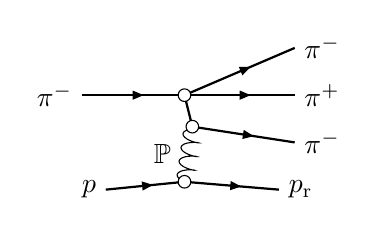
\begin{tikzpicture}[node distance=0.8cm and 1.2cm]
  \coordinate[label=left:{$p$}] (a1);
  \coordinate[right=of a1, xshift=-2mm] (a2);
  \coordinate[right=of a2,label=right:{$\pr$}] (a3);
  \coordinate[above=of a2] (z2);
  \coordinate[above=of z2,yshift=-4mm] (b2);
  \coordinate[below=of z2,yshift=1mm] (z3);
  \coordinate[left=of b2, xshift=-1mm, label=left:{$\pi^-$}] (b1);
  \coordinate[above right=of b2,xshift=2mm,yshift=-2mm, label=right:{$\pi^-$}] (b4);
  \coordinate[      right=of b2,xshift=2mm, label=right:{$\pi^+$}] (b3);
  \coordinate[below right=of b2,xshift=2mm,yshift=2mm, label=right:{$\pi^-$}] (b5);
  \coordinate[below=of b2,yshift=4mm,xshift=1mm] (d2);

  \draw[scalar]  (a1) -- (z3);
  \draw[scalar]  (z3) -- (a3);
  % \draw[scalar]  (b2) -- node[label=left:{$\mathbb{P}$}] {} (a2);
  % \draw[thin,<-] ($(a2)+(0.2,0.2)$) -- node[label={right,xshift=-1mm}:{$t$}] {} ($(b2)+(0.2,-0.5)$);
  \draw[scalar]  (b1) -- (b2);
  \draw[thick]  (b2) -- (d2);
  % pions in final state
  \draw[scalar]  (b2) -- (b4);
  \draw[scalar]  (b2) -- (b3);
  % bachelor
  \draw[scalar]  (d2) -- (b5);
  \draw[gluon]   (z3) -- node[left, xshift=-1mm] {$\Po$} (d2);

  \draw[black,fill=white] (b2) circle [radius=0.08];
  \draw[black,fill=white] (d2) circle [radius=0.08];
  \draw[black,fill=white] (z3) circle [radius=0.08];

\end{tikzpicture}
\end{document}
